\documentclass[twoside]{book}

% Packages required by doxygen
\usepackage{calc}
\usepackage{doxygen}
\usepackage{graphicx}
\usepackage[utf8]{inputenc}
\usepackage{makeidx}
\usepackage{multicol}
\usepackage{multirow}
\usepackage{textcomp}
\usepackage[table]{xcolor}

% Font selection
\usepackage[T1]{fontenc}
\usepackage{mathptmx}
\usepackage[scaled=.90]{helvet}
\usepackage{courier}
\usepackage{amssymb}
\usepackage{sectsty}
\renewcommand{\familydefault}{\sfdefault}
\allsectionsfont{%
  \fontseries{bc}\selectfont%
  \color{darkgray}%
}
\renewcommand{\DoxyLabelFont}{%
  \fontseries{bc}\selectfont%
  \color{darkgray}%
}

% Page & text layout
\usepackage{geometry}
\geometry{%
  a4paper,%
  top=2.5cm,%
  bottom=2.5cm,%
  left=2.5cm,%
  right=2.5cm%
}
\tolerance=750
\hfuzz=15pt
\hbadness=750
\setlength{\emergencystretch}{15pt}
\setlength{\parindent}{0cm}
\setlength{\parskip}{0.2cm}
\makeatletter
\renewcommand{\paragraph}{%
  \@startsection{paragraph}{4}{0ex}{-1.0ex}{1.0ex}{%
    \normalfont\normalsize\bfseries\SS@parafont%
  }%
}
\renewcommand{\subparagraph}{%
  \@startsection{subparagraph}{5}{0ex}{-1.0ex}{1.0ex}{%
    \normalfont\normalsize\bfseries\SS@subparafont%
  }%
}
\makeatother

% Headers & footers
\usepackage{fancyhdr}
\pagestyle{fancyplain}
\fancyhead[LE]{\fancyplain{}{\bfseries\thepage}}
\fancyhead[CE]{\fancyplain{}{}}
\fancyhead[RE]{\fancyplain{}{\bfseries\leftmark}}
\fancyhead[LO]{\fancyplain{}{\bfseries\rightmark}}
\fancyhead[CO]{\fancyplain{}{}}
\fancyhead[RO]{\fancyplain{}{\bfseries\thepage}}
\fancyfoot[LE]{\fancyplain{}{}}
\fancyfoot[CE]{\fancyplain{}{}}
\fancyfoot[RE]{\fancyplain{}{\bfseries\scriptsize Generated on Thu Jul 16 2015 16\-:31\-:33 for My Project by Doxygen }}
\fancyfoot[LO]{\fancyplain{}{\bfseries\scriptsize Generated on Thu Jul 16 2015 16\-:31\-:33 for My Project by Doxygen }}
\fancyfoot[CO]{\fancyplain{}{}}
\fancyfoot[RO]{\fancyplain{}{}}
\renewcommand{\footrulewidth}{0.4pt}
\renewcommand{\chaptermark}[1]{%
  \markboth{#1}{}%
}
\renewcommand{\sectionmark}[1]{%
  \markright{\thesection\ #1}%
}

% Indices & bibliography
\usepackage{natbib}
\usepackage[titles]{tocloft}
\setcounter{tocdepth}{3}
\setcounter{secnumdepth}{5}
\makeindex

% Hyperlinks (required, but should be loaded last)
\usepackage{ifpdf}
\ifpdf
  \usepackage[pdftex,pagebackref=true]{hyperref}
\else
  \usepackage[ps2pdf,pagebackref=true]{hyperref}
\fi
\hypersetup{%
  colorlinks=true,%
  linkcolor=blue,%
  citecolor=blue,%
  unicode%
}

% Custom commands
\newcommand{\clearemptydoublepage}{%
  \newpage{\pagestyle{empty}\cleardoublepage}%
}


%===== C O N T E N T S =====

\begin{document}

% Titlepage & ToC
\hypersetup{pageanchor=false}
\pagenumbering{roman}
\begin{titlepage}
\vspace*{7cm}
\begin{center}%
{\Large My Project }\\
\vspace*{1cm}
{\large Generated by Doxygen 1.8.6}\\
\vspace*{0.5cm}
{\small Thu Jul 16 2015 16:31:33}\\
\end{center}
\end{titlepage}
\clearemptydoublepage
\tableofcontents
\clearemptydoublepage
\pagenumbering{arabic}
\hypersetup{pageanchor=true}

%--- Begin generated contents ---
\chapter{cs378-\/deque}
\label{md_README}
\hypertarget{md_README}{}
\input{md_README}
\chapter{Hierarchical Index}
\section{Class Hierarchy}
This inheritance list is sorted roughly, but not completely, alphabetically\-:\begin{DoxyCompactList}
\item \contentsline{section}{my\-\_\-deque$<$ T, A $>$\-:\-:const\-\_\-iterator}{\pageref{classmy__deque_1_1const__iterator}}{}
\item \contentsline{section}{my\-\_\-deque$<$ T, A $>$\-:\-:iterator}{\pageref{classmy__deque_1_1iterator}}{}
\item \contentsline{section}{my\-\_\-deque$<$ T, A $>$}{\pageref{classmy__deque}}{}
\item Test\begin{DoxyCompactList}
\item \contentsline{section}{Deque\-\_\-\-Fixture$<$ T $>$}{\pageref{structDeque__Fixture}}{}
\end{DoxyCompactList}
\end{DoxyCompactList}

\chapter{Class Index}
\section{Class List}
Here are the classes, structs, unions and interfaces with brief descriptions\-:\begin{DoxyCompactList}
\item\contentsline{section}{\hyperlink{classmy__deque_1_1const__iterator}{my\-\_\-deque$<$ T, A $>$\-::const\-\_\-iterator} }{\pageref{classmy__deque_1_1const__iterator}}{}
\item\contentsline{section}{\hyperlink{structDeque__Fixture}{Deque\-\_\-\-Fixture$<$ T $>$} }{\pageref{structDeque__Fixture}}{}
\item\contentsline{section}{\hyperlink{classmy__deque_1_1iterator}{my\-\_\-deque$<$ T, A $>$\-::iterator} }{\pageref{classmy__deque_1_1iterator}}{}
\item\contentsline{section}{\hyperlink{classmy__deque}{my\-\_\-deque$<$ T, A $>$} }{\pageref{classmy__deque}}{}
\end{DoxyCompactList}

\chapter{Class Documentation}
\hypertarget{classmy__deque_1_1const__iterator}{\section{my\-\_\-deque$<$ T, A $>$\-:\-:const\-\_\-iterator Class Reference}
\label{classmy__deque_1_1const__iterator}\index{my\-\_\-deque$<$ T, A $>$\-::const\-\_\-iterator@{my\-\_\-deque$<$ T, A $>$\-::const\-\_\-iterator}}
}
\subsection*{Public Types}
\begin{DoxyCompactItemize}
\item 
\hypertarget{classmy__deque_1_1const__iterator_a1a84b424e091e49a4af1c13a38621252}{typedef \\*
std\-::bidirectional\-\_\-iterator\-\_\-tag {\bfseries iterator\-\_\-category}}\label{classmy__deque_1_1const__iterator_a1a84b424e091e49a4af1c13a38621252}

\item 
\hypertarget{classmy__deque_1_1const__iterator_adc8d08cb0b0a1dcb50323ba5ab8fdecb}{typedef my\-\_\-deque\-::value\-\_\-type {\bfseries value\-\_\-type}}\label{classmy__deque_1_1const__iterator_adc8d08cb0b0a1dcb50323ba5ab8fdecb}

\item 
\hypertarget{classmy__deque_1_1const__iterator_abe3b655aa980c8a12ba486058464c91d}{typedef my\-\_\-deque\-::difference\-\_\-type {\bfseries difference\-\_\-type}}\label{classmy__deque_1_1const__iterator_abe3b655aa980c8a12ba486058464c91d}

\item 
\hypertarget{classmy__deque_1_1const__iterator_a6a7d42610f3b7e55f38897c151862071}{typedef my\-\_\-deque\-::const\-\_\-pointer {\bfseries pointer}}\label{classmy__deque_1_1const__iterator_a6a7d42610f3b7e55f38897c151862071}

\item 
\hypertarget{classmy__deque_1_1const__iterator_a37cd7eef8e73e5a65d7a9d16ba6d3ed2}{typedef my\-\_\-deque\-::const\-\_\-reference {\bfseries reference}}\label{classmy__deque_1_1const__iterator_a37cd7eef8e73e5a65d7a9d16ba6d3ed2}

\end{DoxyCompactItemize}
\subsection*{Public Member Functions}
\begin{DoxyCompactItemize}
\item 
\hyperlink{classmy__deque_1_1const__iterator_a5277fb9ed18b511d89077834e3564f3c}{const\-\_\-iterator} (const \hyperlink{classmy__deque}{my\-\_\-deque} $\ast$d, size\-\_\-type i=0)
\item 
reference \hyperlink{classmy__deque_1_1const__iterator_a14715989004b54dc6a1bcd3d2ac78a20}{operator$\ast$} () const 
\item 
pointer \hyperlink{classmy__deque_1_1const__iterator_aef7e08cfcebb0c0932422f420645e1ce}{operator-\/$>$} () const 
\item 
\hyperlink{classmy__deque_1_1const__iterator}{const\-\_\-iterator} \& \hyperlink{classmy__deque_1_1const__iterator_a8bc45a394bb73728fca1ebf90755d662}{operator++} ()
\item 
\hyperlink{classmy__deque_1_1const__iterator}{const\-\_\-iterator} \hyperlink{classmy__deque_1_1const__iterator_adf9ea902391ac993088e7c969c64e4de}{operator++} (int)
\item 
\hyperlink{classmy__deque_1_1const__iterator}{const\-\_\-iterator} \& \hyperlink{classmy__deque_1_1const__iterator_ae5dffda4ac0a8ad59a4954dcdeeb5f98}{operator-\/-\/} ()
\item 
\hyperlink{classmy__deque_1_1const__iterator}{const\-\_\-iterator} \hyperlink{classmy__deque_1_1const__iterator_a83c405a1e0b9672c074aaa933a7127df}{operator-\/-\/} (int)
\item 
\hyperlink{classmy__deque_1_1const__iterator}{const\-\_\-iterator} \& \hyperlink{classmy__deque_1_1const__iterator_a2bbc121cc446855edcb9d20451cae024}{operator+=} (difference\-\_\-type d)
\item 
\hyperlink{classmy__deque_1_1const__iterator}{const\-\_\-iterator} \& \hyperlink{classmy__deque_1_1const__iterator_ab51576a76fd33fd55be87ca4c467dc96}{operator-\/=} (difference\-\_\-type d)
\end{DoxyCompactItemize}
\subsection*{Friends}
\begin{DoxyCompactItemize}
\item 
bool \hyperlink{classmy__deque_1_1const__iterator_a772a728ee48f5cb8904aaae842b0eb82}{operator==} (const \hyperlink{classmy__deque_1_1const__iterator}{const\-\_\-iterator} \&lhs, const \hyperlink{classmy__deque_1_1const__iterator}{const\-\_\-iterator} \&rhs)
\item 
bool \hyperlink{classmy__deque_1_1const__iterator_a12d66edf831aeec4957931d7f7945d90}{operator!=} (const \hyperlink{classmy__deque_1_1const__iterator}{const\-\_\-iterator} \&lhs, const \hyperlink{classmy__deque_1_1const__iterator}{const\-\_\-iterator} \&rhs)
\item 
\hyperlink{classmy__deque_1_1const__iterator}{const\-\_\-iterator} \hyperlink{classmy__deque_1_1const__iterator_ab6ce7b11eff6ef34762c30e4e96a86a0}{operator+} (\hyperlink{classmy__deque_1_1const__iterator}{const\-\_\-iterator} lhs, difference\-\_\-type rhs)
\item 
\hyperlink{classmy__deque_1_1const__iterator}{const\-\_\-iterator} \hyperlink{classmy__deque_1_1const__iterator_a41934331896eac6321161ff28c21fb29}{operator-\/} (\hyperlink{classmy__deque_1_1const__iterator}{const\-\_\-iterator} lhs, difference\-\_\-type rhs)
\end{DoxyCompactItemize}


\subsection{Constructor \& Destructor Documentation}
\hypertarget{classmy__deque_1_1const__iterator_a5277fb9ed18b511d89077834e3564f3c}{\index{my\-\_\-deque\-::const\-\_\-iterator@{my\-\_\-deque\-::const\-\_\-iterator}!const\-\_\-iterator@{const\-\_\-iterator}}
\index{const\-\_\-iterator@{const\-\_\-iterator}!my_deque::const_iterator@{my\-\_\-deque\-::const\-\_\-iterator}}
\subsubsection[{const\-\_\-iterator}]{\setlength{\rightskip}{0pt plus 5cm}template$<$typename T , typename A  = std\-::allocator$<$\-T$>$$>$ {\bf my\-\_\-deque}$<$ T, A $>$\-::const\-\_\-iterator\-::const\-\_\-iterator (
\begin{DoxyParamCaption}
\item[{const {\bf my\-\_\-deque} $\ast$}]{d, }
\item[{size\-\_\-type}]{i = {\ttfamily 0}}
\end{DoxyParamCaption}
)\hspace{0.3cm}{\ttfamily [inline]}}}\label{classmy__deque_1_1const__iterator_a5277fb9ed18b511d89077834e3564f3c}

\begin{DoxyParams}{Parameters}
{\em a} & const \hyperlink{classmy__deque}{my\-\_\-deque} \\
\hline
{\em size\-\_\-type} & \\
\hline
\end{DoxyParams}
\begin{DoxyReturn}{Returns}
a const iterator starting at position given for given deque 
\end{DoxyReturn}


\subsection{Member Function Documentation}
\hypertarget{classmy__deque_1_1const__iterator_a14715989004b54dc6a1bcd3d2ac78a20}{\index{my\-\_\-deque\-::const\-\_\-iterator@{my\-\_\-deque\-::const\-\_\-iterator}!operator$\ast$@{operator$\ast$}}
\index{operator$\ast$@{operator$\ast$}!my_deque::const_iterator@{my\-\_\-deque\-::const\-\_\-iterator}}
\subsubsection[{operator$\ast$}]{\setlength{\rightskip}{0pt plus 5cm}template$<$typename T , typename A  = std\-::allocator$<$\-T$>$$>$ reference {\bf my\-\_\-deque}$<$ T, A $>$\-::const\-\_\-iterator\-::operator$\ast$ (
\begin{DoxyParamCaption}
{}
\end{DoxyParamCaption}
) const\hspace{0.3cm}{\ttfamily [inline]}}}\label{classmy__deque_1_1const__iterator_a14715989004b54dc6a1bcd3d2ac78a20}
\begin{DoxyReturn}{Returns}
reference to element at current index 
\end{DoxyReturn}
\hypertarget{classmy__deque_1_1const__iterator_a8bc45a394bb73728fca1ebf90755d662}{\index{my\-\_\-deque\-::const\-\_\-iterator@{my\-\_\-deque\-::const\-\_\-iterator}!operator++@{operator++}}
\index{operator++@{operator++}!my_deque::const_iterator@{my\-\_\-deque\-::const\-\_\-iterator}}
\subsubsection[{operator++}]{\setlength{\rightskip}{0pt plus 5cm}template$<$typename T , typename A  = std\-::allocator$<$\-T$>$$>$ {\bf const\-\_\-iterator}\& {\bf my\-\_\-deque}$<$ T, A $>$\-::const\-\_\-iterator\-::operator++ (
\begin{DoxyParamCaption}
{}
\end{DoxyParamCaption}
)\hspace{0.3cm}{\ttfamily [inline]}}}\label{classmy__deque_1_1const__iterator_a8bc45a394bb73728fca1ebf90755d662}
pre-\/increment \begin{DoxyReturn}{Returns}
const iterator incremented once 
\end{DoxyReturn}
\hypertarget{classmy__deque_1_1const__iterator_adf9ea902391ac993088e7c969c64e4de}{\index{my\-\_\-deque\-::const\-\_\-iterator@{my\-\_\-deque\-::const\-\_\-iterator}!operator++@{operator++}}
\index{operator++@{operator++}!my_deque::const_iterator@{my\-\_\-deque\-::const\-\_\-iterator}}
\subsubsection[{operator++}]{\setlength{\rightskip}{0pt plus 5cm}template$<$typename T , typename A  = std\-::allocator$<$\-T$>$$>$ {\bf const\-\_\-iterator} {\bf my\-\_\-deque}$<$ T, A $>$\-::const\-\_\-iterator\-::operator++ (
\begin{DoxyParamCaption}
\item[{int}]{}
\end{DoxyParamCaption}
)\hspace{0.3cm}{\ttfamily [inline]}}}\label{classmy__deque_1_1const__iterator_adf9ea902391ac993088e7c969c64e4de}
post-\/increment \begin{DoxyReturn}{Returns}
const iterator incremented once 
\end{DoxyReturn}
\hypertarget{classmy__deque_1_1const__iterator_a2bbc121cc446855edcb9d20451cae024}{\index{my\-\_\-deque\-::const\-\_\-iterator@{my\-\_\-deque\-::const\-\_\-iterator}!operator+=@{operator+=}}
\index{operator+=@{operator+=}!my_deque::const_iterator@{my\-\_\-deque\-::const\-\_\-iterator}}
\subsubsection[{operator+=}]{\setlength{\rightskip}{0pt plus 5cm}template$<$typename T , typename A  = std\-::allocator$<$\-T$>$$>$ {\bf const\-\_\-iterator}\& {\bf my\-\_\-deque}$<$ T, A $>$\-::const\-\_\-iterator\-::operator+= (
\begin{DoxyParamCaption}
\item[{difference\-\_\-type}]{d}
\end{DoxyParamCaption}
)\hspace{0.3cm}{\ttfamily [inline]}}}\label{classmy__deque_1_1const__iterator_a2bbc121cc446855edcb9d20451cae024}

\begin{DoxyParams}{Parameters}
{\em difference} & type \\
\hline
\end{DoxyParams}
\begin{DoxyReturn}{Returns}
const iterator incremented by that many 
\end{DoxyReturn}
\hypertarget{classmy__deque_1_1const__iterator_ae5dffda4ac0a8ad59a4954dcdeeb5f98}{\index{my\-\_\-deque\-::const\-\_\-iterator@{my\-\_\-deque\-::const\-\_\-iterator}!operator-\/-\/@{operator-\/-\/}}
\index{operator-\/-\/@{operator-\/-\/}!my_deque::const_iterator@{my\-\_\-deque\-::const\-\_\-iterator}}
\subsubsection[{operator-\/-\/}]{\setlength{\rightskip}{0pt plus 5cm}template$<$typename T , typename A  = std\-::allocator$<$\-T$>$$>$ {\bf const\-\_\-iterator}\& {\bf my\-\_\-deque}$<$ T, A $>$\-::const\-\_\-iterator\-::operator-\/-\/ (
\begin{DoxyParamCaption}
{}
\end{DoxyParamCaption}
)\hspace{0.3cm}{\ttfamily [inline]}}}\label{classmy__deque_1_1const__iterator_ae5dffda4ac0a8ad59a4954dcdeeb5f98}
pre-\/decrement \begin{DoxyReturn}{Returns}
const iterator decremented once 
\end{DoxyReturn}
\hypertarget{classmy__deque_1_1const__iterator_a83c405a1e0b9672c074aaa933a7127df}{\index{my\-\_\-deque\-::const\-\_\-iterator@{my\-\_\-deque\-::const\-\_\-iterator}!operator-\/-\/@{operator-\/-\/}}
\index{operator-\/-\/@{operator-\/-\/}!my_deque::const_iterator@{my\-\_\-deque\-::const\-\_\-iterator}}
\subsubsection[{operator-\/-\/}]{\setlength{\rightskip}{0pt plus 5cm}template$<$typename T , typename A  = std\-::allocator$<$\-T$>$$>$ {\bf const\-\_\-iterator} {\bf my\-\_\-deque}$<$ T, A $>$\-::const\-\_\-iterator\-::operator-\/-\/ (
\begin{DoxyParamCaption}
\item[{int}]{}
\end{DoxyParamCaption}
)\hspace{0.3cm}{\ttfamily [inline]}}}\label{classmy__deque_1_1const__iterator_a83c405a1e0b9672c074aaa933a7127df}
post-\/decrement \begin{DoxyReturn}{Returns}
const iterator decremented once 
\end{DoxyReturn}
\hypertarget{classmy__deque_1_1const__iterator_ab51576a76fd33fd55be87ca4c467dc96}{\index{my\-\_\-deque\-::const\-\_\-iterator@{my\-\_\-deque\-::const\-\_\-iterator}!operator-\/=@{operator-\/=}}
\index{operator-\/=@{operator-\/=}!my_deque::const_iterator@{my\-\_\-deque\-::const\-\_\-iterator}}
\subsubsection[{operator-\/=}]{\setlength{\rightskip}{0pt plus 5cm}template$<$typename T , typename A  = std\-::allocator$<$\-T$>$$>$ {\bf const\-\_\-iterator}\& {\bf my\-\_\-deque}$<$ T, A $>$\-::const\-\_\-iterator\-::operator-\/= (
\begin{DoxyParamCaption}
\item[{difference\-\_\-type}]{d}
\end{DoxyParamCaption}
)\hspace{0.3cm}{\ttfamily [inline]}}}\label{classmy__deque_1_1const__iterator_ab51576a76fd33fd55be87ca4c467dc96}

\begin{DoxyParams}{Parameters}
{\em difference} & type \\
\hline
\end{DoxyParams}
\begin{DoxyReturn}{Returns}
const iterator decremented by that many 
\end{DoxyReturn}
\hypertarget{classmy__deque_1_1const__iterator_aef7e08cfcebb0c0932422f420645e1ce}{\index{my\-\_\-deque\-::const\-\_\-iterator@{my\-\_\-deque\-::const\-\_\-iterator}!operator-\/$>$@{operator-\/$>$}}
\index{operator-\/$>$@{operator-\/$>$}!my_deque::const_iterator@{my\-\_\-deque\-::const\-\_\-iterator}}
\subsubsection[{operator-\/$>$}]{\setlength{\rightskip}{0pt plus 5cm}template$<$typename T , typename A  = std\-::allocator$<$\-T$>$$>$ pointer {\bf my\-\_\-deque}$<$ T, A $>$\-::const\-\_\-iterator\-::operator-\/$>$ (
\begin{DoxyParamCaption}
{}
\end{DoxyParamCaption}
) const\hspace{0.3cm}{\ttfamily [inline]}}}\label{classmy__deque_1_1const__iterator_aef7e08cfcebb0c0932422f420645e1ce}
@ return pointer to this 

\subsection{Friends And Related Function Documentation}
\hypertarget{classmy__deque_1_1const__iterator_a12d66edf831aeec4957931d7f7945d90}{\index{my\-\_\-deque\-::const\-\_\-iterator@{my\-\_\-deque\-::const\-\_\-iterator}!operator!=@{operator!=}}
\index{operator!=@{operator!=}!my_deque::const_iterator@{my\-\_\-deque\-::const\-\_\-iterator}}
\subsubsection[{operator!=}]{\setlength{\rightskip}{0pt plus 5cm}template$<$typename T , typename A  = std\-::allocator$<$\-T$>$$>$ bool operator!= (
\begin{DoxyParamCaption}
\item[{const {\bf const\-\_\-iterator} \&}]{lhs, }
\item[{const {\bf const\-\_\-iterator} \&}]{rhs}
\end{DoxyParamCaption}
)\hspace{0.3cm}{\ttfamily [friend]}}}\label{classmy__deque_1_1const__iterator_a12d66edf831aeec4957931d7f7945d90}

\begin{DoxyParams}{Parameters}
{\em two} & iterators \\
\hline
\end{DoxyParams}
\begin{DoxyReturn}{Returns}
true if the iterators are not equal 
\end{DoxyReturn}
\hypertarget{classmy__deque_1_1const__iterator_ab6ce7b11eff6ef34762c30e4e96a86a0}{\index{my\-\_\-deque\-::const\-\_\-iterator@{my\-\_\-deque\-::const\-\_\-iterator}!operator+@{operator+}}
\index{operator+@{operator+}!my_deque::const_iterator@{my\-\_\-deque\-::const\-\_\-iterator}}
\subsubsection[{operator+}]{\setlength{\rightskip}{0pt plus 5cm}template$<$typename T , typename A  = std\-::allocator$<$\-T$>$$>$ {\bf const\-\_\-iterator} operator+ (
\begin{DoxyParamCaption}
\item[{{\bf const\-\_\-iterator}}]{lhs, }
\item[{difference\-\_\-type}]{rhs}
\end{DoxyParamCaption}
)\hspace{0.3cm}{\ttfamily [friend]}}}\label{classmy__deque_1_1const__iterator_ab6ce7b11eff6ef34762c30e4e96a86a0}

\begin{DoxyParams}{Parameters}
{\em a} & const iterator \\
\hline
{\em a} & difference type \\
\hline
\end{DoxyParams}
\begin{DoxyReturn}{Returns}
the iterator position advanced 
\end{DoxyReturn}
\hypertarget{classmy__deque_1_1const__iterator_a41934331896eac6321161ff28c21fb29}{\index{my\-\_\-deque\-::const\-\_\-iterator@{my\-\_\-deque\-::const\-\_\-iterator}!operator-\/@{operator-\/}}
\index{operator-\/@{operator-\/}!my_deque::const_iterator@{my\-\_\-deque\-::const\-\_\-iterator}}
\subsubsection[{operator-\/}]{\setlength{\rightskip}{0pt plus 5cm}template$<$typename T , typename A  = std\-::allocator$<$\-T$>$$>$ {\bf const\-\_\-iterator} operator-\/ (
\begin{DoxyParamCaption}
\item[{{\bf const\-\_\-iterator}}]{lhs, }
\item[{difference\-\_\-type}]{rhs}
\end{DoxyParamCaption}
)\hspace{0.3cm}{\ttfamily [friend]}}}\label{classmy__deque_1_1const__iterator_a41934331896eac6321161ff28c21fb29}

\begin{DoxyParams}{Parameters}
{\em a} & const iterator \\
\hline
{\em difference} & type \\
\hline
\end{DoxyParams}
\begin{DoxyReturn}{Returns}
iterator decremented by difference type 
\end{DoxyReturn}
\hypertarget{classmy__deque_1_1const__iterator_a772a728ee48f5cb8904aaae842b0eb82}{\index{my\-\_\-deque\-::const\-\_\-iterator@{my\-\_\-deque\-::const\-\_\-iterator}!operator==@{operator==}}
\index{operator==@{operator==}!my_deque::const_iterator@{my\-\_\-deque\-::const\-\_\-iterator}}
\subsubsection[{operator==}]{\setlength{\rightskip}{0pt plus 5cm}template$<$typename T , typename A  = std\-::allocator$<$\-T$>$$>$ bool operator== (
\begin{DoxyParamCaption}
\item[{const {\bf const\-\_\-iterator} \&}]{lhs, }
\item[{const {\bf const\-\_\-iterator} \&}]{rhs}
\end{DoxyParamCaption}
)\hspace{0.3cm}{\ttfamily [friend]}}}\label{classmy__deque_1_1const__iterator_a772a728ee48f5cb8904aaae842b0eb82}

\begin{DoxyParams}{Parameters}
{\em two} & const iterators \\
\hline
\end{DoxyParams}
\begin{DoxyReturn}{Returns}
true if the iterators are equal 
\end{DoxyReturn}


The documentation for this class was generated from the following file\-:\begin{DoxyCompactItemize}
\item 
Deque.\-h\end{DoxyCompactItemize}

\hypertarget{structDeque__Fixture}{\section{Deque\-\_\-\-Fixture$<$ T $>$ Struct Template Reference}
\label{structDeque__Fixture}\index{Deque\-\_\-\-Fixture$<$ T $>$@{Deque\-\_\-\-Fixture$<$ T $>$}}
}
Inheritance diagram for Deque\-\_\-\-Fixture$<$ T $>$\-:\begin{figure}[H]
\begin{center}
\leavevmode
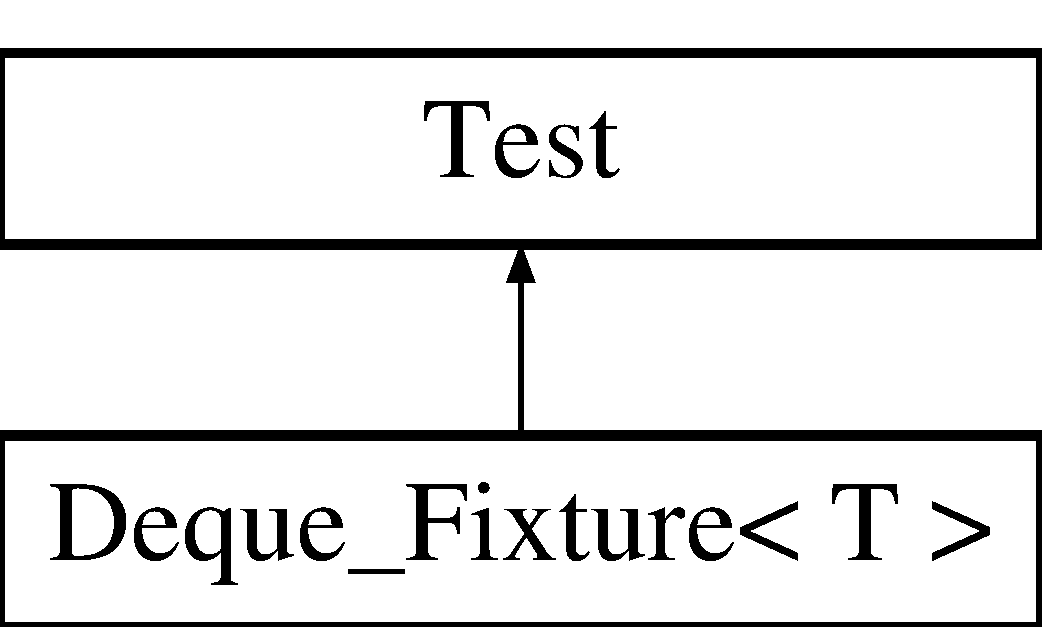
\includegraphics[height=2.000000cm]{structDeque__Fixture}
\end{center}
\end{figure}
\subsection*{Public Types}
\begin{DoxyCompactItemize}
\item 
\hypertarget{structDeque__Fixture_aff55aebc9f3732e55b5e9afae069a6e7}{typedef T {\bfseries deque\-\_\-type}}\label{structDeque__Fixture_aff55aebc9f3732e55b5e9afae069a6e7}

\item 
\hypertarget{structDeque__Fixture_ad3f31d2190bcef2a8809aae173c159e9}{typedef deque\-\_\-type\-::value\-\_\-type {\bfseries value\-\_\-type}}\label{structDeque__Fixture_ad3f31d2190bcef2a8809aae173c159e9}

\end{DoxyCompactItemize}


The documentation for this struct was generated from the following file\-:\begin{DoxyCompactItemize}
\item 
Test\-Deque.\-c++\end{DoxyCompactItemize}

\hypertarget{classmy__deque_1_1iterator}{\section{my\-\_\-deque$<$ T, A $>$\-:\-:iterator Class Reference}
\label{classmy__deque_1_1iterator}\index{my\-\_\-deque$<$ T, A $>$\-::iterator@{my\-\_\-deque$<$ T, A $>$\-::iterator}}
}
\subsection*{Public Types}
\begin{DoxyCompactItemize}
\item 
\hypertarget{classmy__deque_1_1iterator_a0479a0f5fbb1adddafb03cd2c9aaef53}{typedef \\*
std\-::bidirectional\-\_\-iterator\-\_\-tag {\bfseries iterator\-\_\-category}}\label{classmy__deque_1_1iterator_a0479a0f5fbb1adddafb03cd2c9aaef53}

\item 
\hypertarget{classmy__deque_1_1iterator_ac6392e82698893d1802ef0407bd36794}{typedef my\-\_\-deque\-::value\-\_\-type {\bfseries value\-\_\-type}}\label{classmy__deque_1_1iterator_ac6392e82698893d1802ef0407bd36794}

\item 
\hypertarget{classmy__deque_1_1iterator_ac5f62e8566ad92478931c2abd9ac6596}{typedef my\-\_\-deque\-::difference\-\_\-type {\bfseries difference\-\_\-type}}\label{classmy__deque_1_1iterator_ac5f62e8566ad92478931c2abd9ac6596}

\item 
\hypertarget{classmy__deque_1_1iterator_add0e1ed49072422b5aa0ef52303fb86e}{typedef my\-\_\-deque\-::pointer {\bfseries pointer}}\label{classmy__deque_1_1iterator_add0e1ed49072422b5aa0ef52303fb86e}

\item 
\hypertarget{classmy__deque_1_1iterator_ae165ee997a9e18330c593789e9899e57}{typedef my\-\_\-deque\-::reference {\bfseries reference}}\label{classmy__deque_1_1iterator_ae165ee997a9e18330c593789e9899e57}

\end{DoxyCompactItemize}
\subsection*{Public Member Functions}
\begin{DoxyCompactItemize}
\item 
\hyperlink{classmy__deque_1_1iterator_aec0fe04592f368d22e4d80128dc909cb}{iterator} (\hyperlink{classmy__deque}{my\-\_\-deque} $\ast$d, size\-\_\-type i=0)
\item 
reference \hyperlink{classmy__deque_1_1iterator_a12632f02814bba64ca79f42edc0e1497}{operator$\ast$} () const 
\item 
pointer \hyperlink{classmy__deque_1_1iterator_a064f5b1faf5a72113083425133de9a41}{operator-\/$>$} () const 
\item 
\hyperlink{classmy__deque_1_1iterator}{iterator} \& \hyperlink{classmy__deque_1_1iterator_ab2a00619614e204eedb184112a56016e}{operator++} ()
\item 
\hyperlink{classmy__deque_1_1iterator}{iterator} \hyperlink{classmy__deque_1_1iterator_a57f6ac4aef7215ca67b6e05eeda29ee4}{operator++} (int)
\item 
\hyperlink{classmy__deque_1_1iterator}{iterator} \& \hyperlink{classmy__deque_1_1iterator_a278cab96c03498e55ba1aa4e05f1538e}{operator-\/-\/} ()
\item 
\hyperlink{classmy__deque_1_1iterator}{iterator} \hyperlink{classmy__deque_1_1iterator_a5bef4b6332aecf7dcda57cee9a1fdc70}{operator-\/-\/} (int)
\item 
\hyperlink{classmy__deque_1_1iterator}{iterator} \& \hyperlink{classmy__deque_1_1iterator_ad17b4f6e8be4d8242ad4572d62beff82}{operator+=} (difference\-\_\-type d)
\item 
\hyperlink{classmy__deque_1_1iterator}{iterator} \& \hyperlink{classmy__deque_1_1iterator_a13c056d48543734a23a9de09fd652868}{operator-\/=} (difference\-\_\-type d)
\end{DoxyCompactItemize}
\subsection*{Friends}
\begin{DoxyCompactItemize}
\item 
bool \hyperlink{classmy__deque_1_1iterator_a27d0df37bd079bf4e62faa0b468b060c}{operator==} (const \hyperlink{classmy__deque_1_1iterator}{iterator} \&lhs, const \hyperlink{classmy__deque_1_1iterator}{iterator} \&rhs)
\item 
bool \hyperlink{classmy__deque_1_1iterator_aad2b3926ed1e2db6f22ca3117766181b}{operator!=} (const \hyperlink{classmy__deque_1_1iterator}{iterator} \&lhs, const \hyperlink{classmy__deque_1_1iterator}{iterator} \&rhs)
\item 
\hyperlink{classmy__deque_1_1iterator}{iterator} \hyperlink{classmy__deque_1_1iterator_aaf128f38c16b5a8284f51a9c69f6fd77}{operator+} (\hyperlink{classmy__deque_1_1iterator}{iterator} lhs, difference\-\_\-type rhs)
\item 
\hyperlink{classmy__deque_1_1iterator}{iterator} \hyperlink{classmy__deque_1_1iterator_ab8892736ecb2ffe5f6b9ac9b9dbb60c0}{operator-\/} (\hyperlink{classmy__deque_1_1iterator}{iterator} lhs, difference\-\_\-type rhs)
\end{DoxyCompactItemize}


\subsection{Constructor \& Destructor Documentation}
\hypertarget{classmy__deque_1_1iterator_aec0fe04592f368d22e4d80128dc909cb}{\index{my\-\_\-deque\-::iterator@{my\-\_\-deque\-::iterator}!iterator@{iterator}}
\index{iterator@{iterator}!my_deque::iterator@{my\-\_\-deque\-::iterator}}
\subsubsection[{iterator}]{\setlength{\rightskip}{0pt plus 5cm}template$<$typename T , typename A  = std\-::allocator$<$\-T$>$$>$ {\bf my\-\_\-deque}$<$ T, A $>$\-::iterator\-::iterator (
\begin{DoxyParamCaption}
\item[{{\bf my\-\_\-deque} $\ast$}]{d, }
\item[{size\-\_\-type}]{i = {\ttfamily 0}}
\end{DoxyParamCaption}
)\hspace{0.3cm}{\ttfamily [inline]}}}\label{classmy__deque_1_1iterator_aec0fe04592f368d22e4d80128dc909cb}

\begin{DoxyParams}{Parameters}
{\em a} & my deque \\
\hline
{\em a} & size type set iterator on deque at position given \\
\hline
\end{DoxyParams}


\subsection{Member Function Documentation}
\hypertarget{classmy__deque_1_1iterator_a12632f02814bba64ca79f42edc0e1497}{\index{my\-\_\-deque\-::iterator@{my\-\_\-deque\-::iterator}!operator$\ast$@{operator$\ast$}}
\index{operator$\ast$@{operator$\ast$}!my_deque::iterator@{my\-\_\-deque\-::iterator}}
\subsubsection[{operator$\ast$}]{\setlength{\rightskip}{0pt plus 5cm}template$<$typename T , typename A  = std\-::allocator$<$\-T$>$$>$ reference {\bf my\-\_\-deque}$<$ T, A $>$\-::iterator\-::operator$\ast$ (
\begin{DoxyParamCaption}
{}
\end{DoxyParamCaption}
) const\hspace{0.3cm}{\ttfamily [inline]}}}\label{classmy__deque_1_1iterator_a12632f02814bba64ca79f42edc0e1497}
\begin{DoxyReturn}{Returns}
a reference to element at that position 
\end{DoxyReturn}
\hypertarget{classmy__deque_1_1iterator_ab2a00619614e204eedb184112a56016e}{\index{my\-\_\-deque\-::iterator@{my\-\_\-deque\-::iterator}!operator++@{operator++}}
\index{operator++@{operator++}!my_deque::iterator@{my\-\_\-deque\-::iterator}}
\subsubsection[{operator++}]{\setlength{\rightskip}{0pt plus 5cm}template$<$typename T , typename A  = std\-::allocator$<$\-T$>$$>$ {\bf iterator}\& {\bf my\-\_\-deque}$<$ T, A $>$\-::iterator\-::operator++ (
\begin{DoxyParamCaption}
{}
\end{DoxyParamCaption}
)\hspace{0.3cm}{\ttfamily [inline]}}}\label{classmy__deque_1_1iterator_ab2a00619614e204eedb184112a56016e}
pre-\/increment iterator by one to next position \hypertarget{classmy__deque_1_1iterator_a57f6ac4aef7215ca67b6e05eeda29ee4}{\index{my\-\_\-deque\-::iterator@{my\-\_\-deque\-::iterator}!operator++@{operator++}}
\index{operator++@{operator++}!my_deque::iterator@{my\-\_\-deque\-::iterator}}
\subsubsection[{operator++}]{\setlength{\rightskip}{0pt plus 5cm}template$<$typename T , typename A  = std\-::allocator$<$\-T$>$$>$ {\bf iterator} {\bf my\-\_\-deque}$<$ T, A $>$\-::iterator\-::operator++ (
\begin{DoxyParamCaption}
\item[{int}]{}
\end{DoxyParamCaption}
)\hspace{0.3cm}{\ttfamily [inline]}}}\label{classmy__deque_1_1iterator_a57f6ac4aef7215ca67b6e05eeda29ee4}
post-\/increment iterator by one to next position \hypertarget{classmy__deque_1_1iterator_ad17b4f6e8be4d8242ad4572d62beff82}{\index{my\-\_\-deque\-::iterator@{my\-\_\-deque\-::iterator}!operator+=@{operator+=}}
\index{operator+=@{operator+=}!my_deque::iterator@{my\-\_\-deque\-::iterator}}
\subsubsection[{operator+=}]{\setlength{\rightskip}{0pt plus 5cm}template$<$typename T , typename A  = std\-::allocator$<$\-T$>$$>$ {\bf iterator}\& {\bf my\-\_\-deque}$<$ T, A $>$\-::iterator\-::operator+= (
\begin{DoxyParamCaption}
\item[{difference\-\_\-type}]{d}
\end{DoxyParamCaption}
)\hspace{0.3cm}{\ttfamily [inline]}}}\label{classmy__deque_1_1iterator_ad17b4f6e8be4d8242ad4572d62beff82}
increment iterator by value given \hypertarget{classmy__deque_1_1iterator_a278cab96c03498e55ba1aa4e05f1538e}{\index{my\-\_\-deque\-::iterator@{my\-\_\-deque\-::iterator}!operator-\/-\/@{operator-\/-\/}}
\index{operator-\/-\/@{operator-\/-\/}!my_deque::iterator@{my\-\_\-deque\-::iterator}}
\subsubsection[{operator-\/-\/}]{\setlength{\rightskip}{0pt plus 5cm}template$<$typename T , typename A  = std\-::allocator$<$\-T$>$$>$ {\bf iterator}\& {\bf my\-\_\-deque}$<$ T, A $>$\-::iterator\-::operator-\/-\/ (
\begin{DoxyParamCaption}
{}
\end{DoxyParamCaption}
)\hspace{0.3cm}{\ttfamily [inline]}}}\label{classmy__deque_1_1iterator_a278cab96c03498e55ba1aa4e05f1538e}
pre-\/decrement iterator to previous position \hypertarget{classmy__deque_1_1iterator_a5bef4b6332aecf7dcda57cee9a1fdc70}{\index{my\-\_\-deque\-::iterator@{my\-\_\-deque\-::iterator}!operator-\/-\/@{operator-\/-\/}}
\index{operator-\/-\/@{operator-\/-\/}!my_deque::iterator@{my\-\_\-deque\-::iterator}}
\subsubsection[{operator-\/-\/}]{\setlength{\rightskip}{0pt plus 5cm}template$<$typename T , typename A  = std\-::allocator$<$\-T$>$$>$ {\bf iterator} {\bf my\-\_\-deque}$<$ T, A $>$\-::iterator\-::operator-\/-\/ (
\begin{DoxyParamCaption}
\item[{int}]{}
\end{DoxyParamCaption}
)\hspace{0.3cm}{\ttfamily [inline]}}}\label{classmy__deque_1_1iterator_a5bef4b6332aecf7dcda57cee9a1fdc70}
post-\/decrement iterator to previous position \hypertarget{classmy__deque_1_1iterator_a13c056d48543734a23a9de09fd652868}{\index{my\-\_\-deque\-::iterator@{my\-\_\-deque\-::iterator}!operator-\/=@{operator-\/=}}
\index{operator-\/=@{operator-\/=}!my_deque::iterator@{my\-\_\-deque\-::iterator}}
\subsubsection[{operator-\/=}]{\setlength{\rightskip}{0pt plus 5cm}template$<$typename T , typename A  = std\-::allocator$<$\-T$>$$>$ {\bf iterator}\& {\bf my\-\_\-deque}$<$ T, A $>$\-::iterator\-::operator-\/= (
\begin{DoxyParamCaption}
\item[{difference\-\_\-type}]{d}
\end{DoxyParamCaption}
)\hspace{0.3cm}{\ttfamily [inline]}}}\label{classmy__deque_1_1iterator_a13c056d48543734a23a9de09fd652868}
decrement iterator by value given \hypertarget{classmy__deque_1_1iterator_a064f5b1faf5a72113083425133de9a41}{\index{my\-\_\-deque\-::iterator@{my\-\_\-deque\-::iterator}!operator-\/$>$@{operator-\/$>$}}
\index{operator-\/$>$@{operator-\/$>$}!my_deque::iterator@{my\-\_\-deque\-::iterator}}
\subsubsection[{operator-\/$>$}]{\setlength{\rightskip}{0pt plus 5cm}template$<$typename T , typename A  = std\-::allocator$<$\-T$>$$>$ pointer {\bf my\-\_\-deque}$<$ T, A $>$\-::iterator\-::operator-\/$>$ (
\begin{DoxyParamCaption}
{}
\end{DoxyParamCaption}
) const\hspace{0.3cm}{\ttfamily [inline]}}}\label{classmy__deque_1_1iterator_a064f5b1faf5a72113083425133de9a41}

\begin{DoxyParams}{Parameters}
{\em return} & pointer to this \\
\hline
\end{DoxyParams}


\subsection{Friends And Related Function Documentation}
\hypertarget{classmy__deque_1_1iterator_aad2b3926ed1e2db6f22ca3117766181b}{\index{my\-\_\-deque\-::iterator@{my\-\_\-deque\-::iterator}!operator!=@{operator!=}}
\index{operator!=@{operator!=}!my_deque::iterator@{my\-\_\-deque\-::iterator}}
\subsubsection[{operator!=}]{\setlength{\rightskip}{0pt plus 5cm}template$<$typename T , typename A  = std\-::allocator$<$\-T$>$$>$ bool operator!= (
\begin{DoxyParamCaption}
\item[{const {\bf iterator} \&}]{lhs, }
\item[{const {\bf iterator} \&}]{rhs}
\end{DoxyParamCaption}
)\hspace{0.3cm}{\ttfamily [friend]}}}\label{classmy__deque_1_1iterator_aad2b3926ed1e2db6f22ca3117766181b}

\begin{DoxyParams}{Parameters}
{\em take} & in two iterators \\
\hline
\end{DoxyParams}
\begin{DoxyReturn}{Returns}
true if they are not equal 
\end{DoxyReturn}
\hypertarget{classmy__deque_1_1iterator_aaf128f38c16b5a8284f51a9c69f6fd77}{\index{my\-\_\-deque\-::iterator@{my\-\_\-deque\-::iterator}!operator+@{operator+}}
\index{operator+@{operator+}!my_deque::iterator@{my\-\_\-deque\-::iterator}}
\subsubsection[{operator+}]{\setlength{\rightskip}{0pt plus 5cm}template$<$typename T , typename A  = std\-::allocator$<$\-T$>$$>$ {\bf iterator} operator+ (
\begin{DoxyParamCaption}
\item[{{\bf iterator}}]{lhs, }
\item[{difference\-\_\-type}]{rhs}
\end{DoxyParamCaption}
)\hspace{0.3cm}{\ttfamily [friend]}}}\label{classmy__deque_1_1iterator_aaf128f38c16b5a8284f51a9c69f6fd77}

\begin{DoxyParams}{Parameters}
{\em iterator} & \\
\hline
{\em difference} & type \\
\hline
\end{DoxyParams}
\begin{DoxyReturn}{Returns}
the iterator advanced difference\-\_\-type number of places (sum) 
\end{DoxyReturn}
\hypertarget{classmy__deque_1_1iterator_ab8892736ecb2ffe5f6b9ac9b9dbb60c0}{\index{my\-\_\-deque\-::iterator@{my\-\_\-deque\-::iterator}!operator-\/@{operator-\/}}
\index{operator-\/@{operator-\/}!my_deque::iterator@{my\-\_\-deque\-::iterator}}
\subsubsection[{operator-\/}]{\setlength{\rightskip}{0pt plus 5cm}template$<$typename T , typename A  = std\-::allocator$<$\-T$>$$>$ {\bf iterator} operator-\/ (
\begin{DoxyParamCaption}
\item[{{\bf iterator}}]{lhs, }
\item[{difference\-\_\-type}]{rhs}
\end{DoxyParamCaption}
)\hspace{0.3cm}{\ttfamily [friend]}}}\label{classmy__deque_1_1iterator_ab8892736ecb2ffe5f6b9ac9b9dbb60c0}

\begin{DoxyParams}{Parameters}
{\em iterator} & \\
\hline
{\em difference} & type \\
\hline
\end{DoxyParams}
\begin{DoxyReturn}{Returns}
decremented iterator by number of difference type 
\end{DoxyReturn}
\hypertarget{classmy__deque_1_1iterator_a27d0df37bd079bf4e62faa0b468b060c}{\index{my\-\_\-deque\-::iterator@{my\-\_\-deque\-::iterator}!operator==@{operator==}}
\index{operator==@{operator==}!my_deque::iterator@{my\-\_\-deque\-::iterator}}
\subsubsection[{operator==}]{\setlength{\rightskip}{0pt plus 5cm}template$<$typename T , typename A  = std\-::allocator$<$\-T$>$$>$ bool operator== (
\begin{DoxyParamCaption}
\item[{const {\bf iterator} \&}]{lhs, }
\item[{const {\bf iterator} \&}]{rhs}
\end{DoxyParamCaption}
)\hspace{0.3cm}{\ttfamily [friend]}}}\label{classmy__deque_1_1iterator_a27d0df37bd079bf4e62faa0b468b060c}

\begin{DoxyParams}{Parameters}
{\em take} & in two iterators \\
\hline
\end{DoxyParams}
\begin{DoxyReturn}{Returns}
true if they are equal 
\end{DoxyReturn}


The documentation for this class was generated from the following file\-:\begin{DoxyCompactItemize}
\item 
Deque.\-h\end{DoxyCompactItemize}

\hypertarget{classmy__deque}{\section{my\-\_\-deque$<$ T, A $>$ Class Template Reference}
\label{classmy__deque}\index{my\-\_\-deque$<$ T, A $>$@{my\-\_\-deque$<$ T, A $>$}}
}
\subsection*{Classes}
\begin{DoxyCompactItemize}
\item 
class \hyperlink{classmy__deque_1_1const__iterator}{const\-\_\-iterator}
\item 
class \hyperlink{classmy__deque_1_1iterator}{iterator}
\end{DoxyCompactItemize}
\subsection*{Public Types}
\begin{DoxyCompactItemize}
\item 
\hypertarget{classmy__deque_a34236f0fef930decd11dc683f40a38be}{typedef A {\bfseries allocator\-\_\-type}}\label{classmy__deque_a34236f0fef930decd11dc683f40a38be}

\item 
\hypertarget{classmy__deque_ae9c156c405acc57623a4601ce755596f}{typedef allocator\-\_\-type\-::value\-\_\-type {\bfseries value\-\_\-type}}\label{classmy__deque_ae9c156c405acc57623a4601ce755596f}

\item 
\hypertarget{classmy__deque_a61e5e5317fe72a381ce4d45f09544b02}{typedef allocator\-\_\-type\-::size\-\_\-type {\bfseries size\-\_\-type}}\label{classmy__deque_a61e5e5317fe72a381ce4d45f09544b02}

\item 
\hypertarget{classmy__deque_ac85676cb2492fbc9bbc6f1a30e9d3c73}{typedef \\*
allocator\-\_\-type\-::difference\-\_\-type {\bfseries difference\-\_\-type}}\label{classmy__deque_ac85676cb2492fbc9bbc6f1a30e9d3c73}

\item 
\hypertarget{classmy__deque_a58e82fc365a3b086367479515e1515be}{typedef allocator\-\_\-type\-::pointer {\bfseries pointer}}\label{classmy__deque_a58e82fc365a3b086367479515e1515be}

\item 
\hypertarget{classmy__deque_a8fea5edeb2b2cf3dd1246dc3abf9b71b}{typedef \\*
allocator\-\_\-type\-::const\-\_\-pointer {\bfseries const\-\_\-pointer}}\label{classmy__deque_a8fea5edeb2b2cf3dd1246dc3abf9b71b}

\item 
\hypertarget{classmy__deque_a4c34c14f397b7676445b37c87003116b}{typedef allocator\-\_\-type\-::reference {\bfseries reference}}\label{classmy__deque_a4c34c14f397b7676445b37c87003116b}

\item 
\hypertarget{classmy__deque_ad50d8b378580088cf77fa43f0640e49c}{typedef \\*
allocator\-\_\-type\-::const\-\_\-reference {\bfseries const\-\_\-reference}}\label{classmy__deque_ad50d8b378580088cf77fa43f0640e49c}

\item 
\hypertarget{classmy__deque_a1a55c016646bba79086d90d3cccde143}{typedef A\-::template rebind\\*
$<$ pointer $>$\-::other {\bfseries B}}\label{classmy__deque_a1a55c016646bba79086d90d3cccde143}

\item 
\hypertarget{classmy__deque_a87d923dafdeeadf5c013f69a73a7daa7}{typedef \\*
allocator\-\_\-type\-::template \\*
rebind$<$ T $\ast$ $>$\-::other {\bfseries all\-\_\-pointer}}\label{classmy__deque_a87d923dafdeeadf5c013f69a73a7daa7}

\end{DoxyCompactItemize}
\subsection*{Public Member Functions}
\begin{DoxyCompactItemize}
\item 
\hyperlink{classmy__deque_ad2ac9d80048c55fcc045d2861c73aa1a}{my\-\_\-deque} (const allocator\-\_\-type \&a=allocator\-\_\-type())
\item 
\hyperlink{classmy__deque_aeaf4c625438497a7cd6a670da6c2c08b}{my\-\_\-deque} (size\-\_\-type s, const\-\_\-reference v=value\-\_\-type(), const allocator\-\_\-type \&a=allocator\-\_\-type())
\item 
\hyperlink{classmy__deque_a59015bc46e6096555d631d69dc8fd7e7}{my\-\_\-deque} (const \hyperlink{classmy__deque}{my\-\_\-deque} \&that)
\item 
\hyperlink{classmy__deque_ae22194ee436865a59a7475c339a9c1ca}{$\sim$my\-\_\-deque} ()
\item 
\hyperlink{classmy__deque}{my\-\_\-deque} \& \hyperlink{classmy__deque_aaa103f2058854bb98e500de6305b1564}{operator=} (const \hyperlink{classmy__deque}{my\-\_\-deque} \&rhs)
\item 
reference \hyperlink{classmy__deque_a489b77decf4d424f43092e194d69444f}{operator\mbox{[}$\,$\mbox{]}} (size\-\_\-type index)
\item 
const\-\_\-reference \hyperlink{classmy__deque_ad79fcd9e94dfc5566e1cd0ce606cf208}{operator\mbox{[}$\,$\mbox{]}} (size\-\_\-type index) const 
\item 
reference \hyperlink{classmy__deque_a75106748e6ff8735e40560e7335bd500}{at} (size\-\_\-type index)
\item 
const\-\_\-reference \hyperlink{classmy__deque_a9642816a10e6a6ee1f8a5367987b8ee8}{at} (size\-\_\-type index) const 
\item 
reference \hyperlink{classmy__deque_a1d9aadb5bedc29da86d4323587cd5e4d}{back} ()
\item 
const\-\_\-reference \hyperlink{classmy__deque_ac273f9574a95af619b9f0dcc0d2e89d0}{back} () const 
\item 
\hyperlink{classmy__deque_1_1iterator}{iterator} \hyperlink{classmy__deque_aef8cac69d47cb1c274896b82ba8f453a}{begin} ()
\item 
\hyperlink{classmy__deque_1_1const__iterator}{const\-\_\-iterator} \hyperlink{classmy__deque_a8612539eff4ee446f85ffb30abf91a69}{begin} () const 
\item 
void \hyperlink{classmy__deque_aa29f90c63cde532f5fc169e8e66b514c}{clear} ()
\item 
bool \hyperlink{classmy__deque_a2b4f029c47afbdbf057639c5a6816d6c}{empty} () const 
\item 
\hyperlink{classmy__deque_1_1iterator}{iterator} \hyperlink{classmy__deque_a2576ee71790ebe55ac4200c506540bb5}{end} ()
\item 
\hyperlink{classmy__deque_1_1const__iterator}{const\-\_\-iterator} \hyperlink{classmy__deque_af465c3f8483634e4e656d90f8d0d88fb}{end} () const 
\item 
\hyperlink{classmy__deque_1_1iterator}{iterator} \hyperlink{classmy__deque_a68328ee9d14996c56ccac5e9981741d5}{erase} (\hyperlink{classmy__deque_1_1iterator}{iterator} i)
\item 
reference \hyperlink{classmy__deque_a0eae28af0ffdd813d1f94f57d393fdf8}{front} ()
\item 
const\-\_\-reference \hyperlink{classmy__deque_a0f1239043b7339b8237a0c8bc663be6b}{front} () const 
\item 
\hyperlink{classmy__deque_1_1iterator}{iterator} \hyperlink{classmy__deque_a8f6b40ddfb98b9b2fb0f05367e584a20}{insert} (\hyperlink{classmy__deque_1_1iterator}{iterator} it, const\-\_\-reference r)
\item 
void \hyperlink{classmy__deque_a63cc9691ee90701693e948246311c498}{pop\-\_\-back} ()
\item 
void \hyperlink{classmy__deque_a85c322cdc4f629e44abdcf369fdd3dab}{pop\-\_\-front} ()
\item 
void \hyperlink{classmy__deque_a15867a8b57c321dcc8ebb4cfa785d7ca}{push\-\_\-back} (const\-\_\-reference v)
\item 
void \hyperlink{classmy__deque_af8d66a7ed1fd51476ec785228ac76996}{push\-\_\-front} (const\-\_\-reference v)
\item 
void \hyperlink{classmy__deque_a80369f549dcd0a2ea9bc086fc97c8e25}{resize} (size\-\_\-type s, const\-\_\-reference v=value\-\_\-type())
\item 
size\-\_\-type \hyperlink{classmy__deque_a3100498f22d2dfa480b141f8ef7990ca}{size} () const 
\item 
void \hyperlink{classmy__deque_a50f83432394d6d068d4d96a3515d7b79}{swap} (\hyperlink{classmy__deque}{my\-\_\-deque} \&that)
\end{DoxyCompactItemize}
\subsection*{Friends}
\begin{DoxyCompactItemize}
\item 
bool \hyperlink{classmy__deque_aca1e37552707f9d7710a6af82cf1262e}{operator==} (const \hyperlink{classmy__deque}{my\-\_\-deque} \&lhs, const \hyperlink{classmy__deque}{my\-\_\-deque} \&rhs)
\item 
bool \hyperlink{classmy__deque_abd32df1d76a0ab0c1519f65cc4fa1363}{operator$<$} (const \hyperlink{classmy__deque}{my\-\_\-deque} \&lhs, const \hyperlink{classmy__deque}{my\-\_\-deque} \&rhs)
\end{DoxyCompactItemize}


\subsection{Constructor \& Destructor Documentation}
\hypertarget{classmy__deque_ad2ac9d80048c55fcc045d2861c73aa1a}{\index{my\-\_\-deque@{my\-\_\-deque}!my\-\_\-deque@{my\-\_\-deque}}
\index{my\-\_\-deque@{my\-\_\-deque}!my_deque@{my\-\_\-deque}}
\subsubsection[{my\-\_\-deque}]{\setlength{\rightskip}{0pt plus 5cm}template$<$typename T , typename A  = std\-::allocator$<$\-T$>$$>$ {\bf my\-\_\-deque}$<$ T, A $>$\-::{\bf my\-\_\-deque} (
\begin{DoxyParamCaption}
\item[{const allocator\-\_\-type \&}]{a = {\ttfamily allocator\-\_\-type()}}
\end{DoxyParamCaption}
)\hspace{0.3cm}{\ttfamily [inline]}, {\ttfamily [explicit]}}}\label{classmy__deque_ad2ac9d80048c55fcc045d2861c73aa1a}
defaul constructor 
\begin{DoxyParams}{Parameters}
{\em allocator} & type defaulted set everything to 0 \\
\hline
\end{DoxyParams}
\hypertarget{classmy__deque_aeaf4c625438497a7cd6a670da6c2c08b}{\index{my\-\_\-deque@{my\-\_\-deque}!my\-\_\-deque@{my\-\_\-deque}}
\index{my\-\_\-deque@{my\-\_\-deque}!my_deque@{my\-\_\-deque}}
\subsubsection[{my\-\_\-deque}]{\setlength{\rightskip}{0pt plus 5cm}template$<$typename T , typename A  = std\-::allocator$<$\-T$>$$>$ {\bf my\-\_\-deque}$<$ T, A $>$\-::{\bf my\-\_\-deque} (
\begin{DoxyParamCaption}
\item[{size\-\_\-type}]{s, }
\item[{const\-\_\-reference}]{v = {\ttfamily value\-\_\-type()}, }
\item[{const allocator\-\_\-type \&}]{a = {\ttfamily allocator\-\_\-type()}}
\end{DoxyParamCaption}
)\hspace{0.3cm}{\ttfamily [inline]}, {\ttfamily [explicit]}}}\label{classmy__deque_aeaf4c625438497a7cd6a670da6c2c08b}
constructor with given size split size up into rows and columns \hypertarget{classmy__deque_a59015bc46e6096555d631d69dc8fd7e7}{\index{my\-\_\-deque@{my\-\_\-deque}!my\-\_\-deque@{my\-\_\-deque}}
\index{my\-\_\-deque@{my\-\_\-deque}!my_deque@{my\-\_\-deque}}
\subsubsection[{my\-\_\-deque}]{\setlength{\rightskip}{0pt plus 5cm}template$<$typename T , typename A  = std\-::allocator$<$\-T$>$$>$ {\bf my\-\_\-deque}$<$ T, A $>$\-::{\bf my\-\_\-deque} (
\begin{DoxyParamCaption}
\item[{const {\bf my\-\_\-deque}$<$ T, A $>$ \&}]{that}
\end{DoxyParamCaption}
)\hspace{0.3cm}{\ttfamily [inline]}}}\label{classmy__deque_a59015bc46e6096555d631d69dc8fd7e7}
copy constructor 
\begin{DoxyParams}{Parameters}
{\em \hyperlink{classmy__deque}{my\-\_\-deque}} & to be copied \\
\hline
\end{DoxyParams}
\hypertarget{classmy__deque_ae22194ee436865a59a7475c339a9c1ca}{\index{my\-\_\-deque@{my\-\_\-deque}!$\sim$my\-\_\-deque@{$\sim$my\-\_\-deque}}
\index{$\sim$my\-\_\-deque@{$\sim$my\-\_\-deque}!my_deque@{my\-\_\-deque}}
\subsubsection[{$\sim$my\-\_\-deque}]{\setlength{\rightskip}{0pt plus 5cm}template$<$typename T , typename A  = std\-::allocator$<$\-T$>$$>$ {\bf my\-\_\-deque}$<$ T, A $>$\-::$\sim${\bf my\-\_\-deque} (
\begin{DoxyParamCaption}
{}
\end{DoxyParamCaption}
)\hspace{0.3cm}{\ttfamily [inline]}}}\label{classmy__deque_ae22194ee436865a59a7475c339a9c1ca}
destructor if not empty, clear and deallocate space 

\subsection{Member Function Documentation}
\hypertarget{classmy__deque_a75106748e6ff8735e40560e7335bd500}{\index{my\-\_\-deque@{my\-\_\-deque}!at@{at}}
\index{at@{at}!my_deque@{my\-\_\-deque}}
\subsubsection[{at}]{\setlength{\rightskip}{0pt plus 5cm}template$<$typename T , typename A  = std\-::allocator$<$\-T$>$$>$ reference {\bf my\-\_\-deque}$<$ T, A $>$\-::at (
\begin{DoxyParamCaption}
\item[{size\-\_\-type}]{index}
\end{DoxyParamCaption}
)\hspace{0.3cm}{\ttfamily [inline]}}}\label{classmy__deque_a75106748e6ff8735e40560e7335bd500}
\begin{DoxyReturn}{Returns}
reference to value at index 
\end{DoxyReturn}
\hypertarget{classmy__deque_a9642816a10e6a6ee1f8a5367987b8ee8}{\index{my\-\_\-deque@{my\-\_\-deque}!at@{at}}
\index{at@{at}!my_deque@{my\-\_\-deque}}
\subsubsection[{at}]{\setlength{\rightskip}{0pt plus 5cm}template$<$typename T , typename A  = std\-::allocator$<$\-T$>$$>$ const\-\_\-reference {\bf my\-\_\-deque}$<$ T, A $>$\-::at (
\begin{DoxyParamCaption}
\item[{size\-\_\-type}]{index}
\end{DoxyParamCaption}
) const\hspace{0.3cm}{\ttfamily [inline]}}}\label{classmy__deque_a9642816a10e6a6ee1f8a5367987b8ee8}
\begin{DoxyReturn}{Returns}
const reference to value at index 
\end{DoxyReturn}
\hypertarget{classmy__deque_a1d9aadb5bedc29da86d4323587cd5e4d}{\index{my\-\_\-deque@{my\-\_\-deque}!back@{back}}
\index{back@{back}!my_deque@{my\-\_\-deque}}
\subsubsection[{back}]{\setlength{\rightskip}{0pt plus 5cm}template$<$typename T , typename A  = std\-::allocator$<$\-T$>$$>$ reference {\bf my\-\_\-deque}$<$ T, A $>$\-::back (
\begin{DoxyParamCaption}
{}
\end{DoxyParamCaption}
)\hspace{0.3cm}{\ttfamily [inline]}}}\label{classmy__deque_a1d9aadb5bedc29da86d4323587cd5e4d}
\begin{DoxyReturn}{Returns}
the reference to last element has to be end of data, not end of capacity 
\end{DoxyReturn}
\hypertarget{classmy__deque_ac273f9574a95af619b9f0dcc0d2e89d0}{\index{my\-\_\-deque@{my\-\_\-deque}!back@{back}}
\index{back@{back}!my_deque@{my\-\_\-deque}}
\subsubsection[{back}]{\setlength{\rightskip}{0pt plus 5cm}template$<$typename T , typename A  = std\-::allocator$<$\-T$>$$>$ const\-\_\-reference {\bf my\-\_\-deque}$<$ T, A $>$\-::back (
\begin{DoxyParamCaption}
{}
\end{DoxyParamCaption}
) const\hspace{0.3cm}{\ttfamily [inline]}}}\label{classmy__deque_ac273f9574a95af619b9f0dcc0d2e89d0}
\begin{DoxyReturn}{Returns}
const reference to last element 
\end{DoxyReturn}
\hypertarget{classmy__deque_aef8cac69d47cb1c274896b82ba8f453a}{\index{my\-\_\-deque@{my\-\_\-deque}!begin@{begin}}
\index{begin@{begin}!my_deque@{my\-\_\-deque}}
\subsubsection[{begin}]{\setlength{\rightskip}{0pt plus 5cm}template$<$typename T , typename A  = std\-::allocator$<$\-T$>$$>$ {\bf iterator} {\bf my\-\_\-deque}$<$ T, A $>$\-::begin (
\begin{DoxyParamCaption}
{}
\end{DoxyParamCaption}
)\hspace{0.3cm}{\ttfamily [inline]}}}\label{classmy__deque_aef8cac69d47cb1c274896b82ba8f453a}
\begin{DoxyReturn}{Returns}
iterator to beginning position (default) 
\end{DoxyReturn}
\hypertarget{classmy__deque_a8612539eff4ee446f85ffb30abf91a69}{\index{my\-\_\-deque@{my\-\_\-deque}!begin@{begin}}
\index{begin@{begin}!my_deque@{my\-\_\-deque}}
\subsubsection[{begin}]{\setlength{\rightskip}{0pt plus 5cm}template$<$typename T , typename A  = std\-::allocator$<$\-T$>$$>$ {\bf const\-\_\-iterator} {\bf my\-\_\-deque}$<$ T, A $>$\-::begin (
\begin{DoxyParamCaption}
{}
\end{DoxyParamCaption}
) const\hspace{0.3cm}{\ttfamily [inline]}}}\label{classmy__deque_a8612539eff4ee446f85ffb30abf91a69}
\begin{DoxyReturn}{Returns}
constant iterator to beginning position (default) 
\end{DoxyReturn}
\hypertarget{classmy__deque_aa29f90c63cde532f5fc169e8e66b514c}{\index{my\-\_\-deque@{my\-\_\-deque}!clear@{clear}}
\index{clear@{clear}!my_deque@{my\-\_\-deque}}
\subsubsection[{clear}]{\setlength{\rightskip}{0pt plus 5cm}template$<$typename T , typename A  = std\-::allocator$<$\-T$>$$>$ void {\bf my\-\_\-deque}$<$ T, A $>$\-::clear (
\begin{DoxyParamCaption}
{}
\end{DoxyParamCaption}
)\hspace{0.3cm}{\ttfamily [inline]}}}\label{classmy__deque_aa29f90c63cde532f5fc169e8e66b514c}
resize to 0 to clear all data \hypertarget{classmy__deque_a2b4f029c47afbdbf057639c5a6816d6c}{\index{my\-\_\-deque@{my\-\_\-deque}!empty@{empty}}
\index{empty@{empty}!my_deque@{my\-\_\-deque}}
\subsubsection[{empty}]{\setlength{\rightskip}{0pt plus 5cm}template$<$typename T , typename A  = std\-::allocator$<$\-T$>$$>$ bool {\bf my\-\_\-deque}$<$ T, A $>$\-::empty (
\begin{DoxyParamCaption}
{}
\end{DoxyParamCaption}
) const\hspace{0.3cm}{\ttfamily [inline]}}}\label{classmy__deque_a2b4f029c47afbdbf057639c5a6816d6c}
\begin{DoxyReturn}{Returns}
true if \hyperlink{classmy__deque}{my\-\_\-deque} is empty 
\end{DoxyReturn}
\hypertarget{classmy__deque_a2576ee71790ebe55ac4200c506540bb5}{\index{my\-\_\-deque@{my\-\_\-deque}!end@{end}}
\index{end@{end}!my_deque@{my\-\_\-deque}}
\subsubsection[{end}]{\setlength{\rightskip}{0pt plus 5cm}template$<$typename T , typename A  = std\-::allocator$<$\-T$>$$>$ {\bf iterator} {\bf my\-\_\-deque}$<$ T, A $>$\-::end (
\begin{DoxyParamCaption}
{}
\end{DoxyParamCaption}
)\hspace{0.3cm}{\ttfamily [inline]}}}\label{classmy__deque_a2576ee71790ebe55ac4200c506540bb5}
\begin{DoxyReturn}{Returns}
iterator to the end 
\end{DoxyReturn}
\hypertarget{classmy__deque_af465c3f8483634e4e656d90f8d0d88fb}{\index{my\-\_\-deque@{my\-\_\-deque}!end@{end}}
\index{end@{end}!my_deque@{my\-\_\-deque}}
\subsubsection[{end}]{\setlength{\rightskip}{0pt plus 5cm}template$<$typename T , typename A  = std\-::allocator$<$\-T$>$$>$ {\bf const\-\_\-iterator} {\bf my\-\_\-deque}$<$ T, A $>$\-::end (
\begin{DoxyParamCaption}
{}
\end{DoxyParamCaption}
) const\hspace{0.3cm}{\ttfamily [inline]}}}\label{classmy__deque_af465c3f8483634e4e656d90f8d0d88fb}
\begin{DoxyReturn}{Returns}
const iterator to the end 
\end{DoxyReturn}
\hypertarget{classmy__deque_a68328ee9d14996c56ccac5e9981741d5}{\index{my\-\_\-deque@{my\-\_\-deque}!erase@{erase}}
\index{erase@{erase}!my_deque@{my\-\_\-deque}}
\subsubsection[{erase}]{\setlength{\rightskip}{0pt plus 5cm}template$<$typename T , typename A  = std\-::allocator$<$\-T$>$$>$ {\bf iterator} {\bf my\-\_\-deque}$<$ T, A $>$\-::erase (
\begin{DoxyParamCaption}
\item[{{\bf iterator}}]{i}
\end{DoxyParamCaption}
)\hspace{0.3cm}{\ttfamily [inline]}}}\label{classmy__deque_a68328ee9d14996c56ccac5e9981741d5}
$<$your documentation$>$=\char`\"{}\char`\"{}$>$ \hypertarget{classmy__deque_a0eae28af0ffdd813d1f94f57d393fdf8}{\index{my\-\_\-deque@{my\-\_\-deque}!front@{front}}
\index{front@{front}!my_deque@{my\-\_\-deque}}
\subsubsection[{front}]{\setlength{\rightskip}{0pt plus 5cm}template$<$typename T , typename A  = std\-::allocator$<$\-T$>$$>$ reference {\bf my\-\_\-deque}$<$ T, A $>$\-::front (
\begin{DoxyParamCaption}
{}
\end{DoxyParamCaption}
)\hspace{0.3cm}{\ttfamily [inline]}}}\label{classmy__deque_a0eae28af0ffdd813d1f94f57d393fdf8}
\begin{DoxyReturn}{Returns}
reference to the first element 
\end{DoxyReturn}
\hypertarget{classmy__deque_a0f1239043b7339b8237a0c8bc663be6b}{\index{my\-\_\-deque@{my\-\_\-deque}!front@{front}}
\index{front@{front}!my_deque@{my\-\_\-deque}}
\subsubsection[{front}]{\setlength{\rightskip}{0pt plus 5cm}template$<$typename T , typename A  = std\-::allocator$<$\-T$>$$>$ const\-\_\-reference {\bf my\-\_\-deque}$<$ T, A $>$\-::front (
\begin{DoxyParamCaption}
{}
\end{DoxyParamCaption}
) const\hspace{0.3cm}{\ttfamily [inline]}}}\label{classmy__deque_a0f1239043b7339b8237a0c8bc663be6b}
\begin{DoxyReturn}{Returns}
const reference to first element 
\end{DoxyReturn}
\hypertarget{classmy__deque_a8f6b40ddfb98b9b2fb0f05367e584a20}{\index{my\-\_\-deque@{my\-\_\-deque}!insert@{insert}}
\index{insert@{insert}!my_deque@{my\-\_\-deque}}
\subsubsection[{insert}]{\setlength{\rightskip}{0pt plus 5cm}template$<$typename T , typename A  = std\-::allocator$<$\-T$>$$>$ {\bf iterator} {\bf my\-\_\-deque}$<$ T, A $>$\-::insert (
\begin{DoxyParamCaption}
\item[{{\bf iterator}}]{it, }
\item[{const\-\_\-reference}]{r}
\end{DoxyParamCaption}
)\hspace{0.3cm}{\ttfamily [inline]}}}\label{classmy__deque_a8f6b40ddfb98b9b2fb0f05367e584a20}
\begin{DoxyReturn}{Returns}
iterator to given position, but with new value 
\end{DoxyReturn}
\hypertarget{classmy__deque_aaa103f2058854bb98e500de6305b1564}{\index{my\-\_\-deque@{my\-\_\-deque}!operator=@{operator=}}
\index{operator=@{operator=}!my_deque@{my\-\_\-deque}}
\subsubsection[{operator=}]{\setlength{\rightskip}{0pt plus 5cm}template$<$typename T , typename A  = std\-::allocator$<$\-T$>$$>$ {\bf my\-\_\-deque}\& {\bf my\-\_\-deque}$<$ T, A $>$\-::operator= (
\begin{DoxyParamCaption}
\item[{const {\bf my\-\_\-deque}$<$ T, A $>$ \&}]{rhs}
\end{DoxyParamCaption}
)\hspace{0.3cm}{\ttfamily [inline]}}}\label{classmy__deque_aaa103f2058854bb98e500de6305b1564}

\begin{DoxyParams}{Parameters}
{\em \hyperlink{classmy__deque}{my\-\_\-deque}} & \\
\hline
\end{DoxyParams}
\hypertarget{classmy__deque_a489b77decf4d424f43092e194d69444f}{\index{my\-\_\-deque@{my\-\_\-deque}!operator\mbox{[}$\,$\mbox{]}@{operator[]}}
\index{operator\mbox{[}$\,$\mbox{]}@{operator[]}!my_deque@{my\-\_\-deque}}
\subsubsection[{operator[]}]{\setlength{\rightskip}{0pt plus 5cm}template$<$typename T , typename A  = std\-::allocator$<$\-T$>$$>$ reference {\bf my\-\_\-deque}$<$ T, A $>$\-::operator\mbox{[}$\,$\mbox{]} (
\begin{DoxyParamCaption}
\item[{size\-\_\-type}]{index}
\end{DoxyParamCaption}
)\hspace{0.3cm}{\ttfamily [inline]}}}\label{classmy__deque_a489b77decf4d424f43092e194d69444f}
\begin{DoxyReturn}{Returns}
reference to value at index from beginning of data 
\end{DoxyReturn}
\hypertarget{classmy__deque_ad79fcd9e94dfc5566e1cd0ce606cf208}{\index{my\-\_\-deque@{my\-\_\-deque}!operator\mbox{[}$\,$\mbox{]}@{operator[]}}
\index{operator\mbox{[}$\,$\mbox{]}@{operator[]}!my_deque@{my\-\_\-deque}}
\subsubsection[{operator[]}]{\setlength{\rightskip}{0pt plus 5cm}template$<$typename T , typename A  = std\-::allocator$<$\-T$>$$>$ const\-\_\-reference {\bf my\-\_\-deque}$<$ T, A $>$\-::operator\mbox{[}$\,$\mbox{]} (
\begin{DoxyParamCaption}
\item[{size\-\_\-type}]{index}
\end{DoxyParamCaption}
) const\hspace{0.3cm}{\ttfamily [inline]}}}\label{classmy__deque_ad79fcd9e94dfc5566e1cd0ce606cf208}
\begin{DoxyReturn}{Returns}
const reference to value at index from beginning of data 
\end{DoxyReturn}
\hypertarget{classmy__deque_a63cc9691ee90701693e948246311c498}{\index{my\-\_\-deque@{my\-\_\-deque}!pop\-\_\-back@{pop\-\_\-back}}
\index{pop\-\_\-back@{pop\-\_\-back}!my_deque@{my\-\_\-deque}}
\subsubsection[{pop\-\_\-back}]{\setlength{\rightskip}{0pt plus 5cm}template$<$typename T , typename A  = std\-::allocator$<$\-T$>$$>$ void {\bf my\-\_\-deque}$<$ T, A $>$\-::pop\-\_\-back (
\begin{DoxyParamCaption}
{}
\end{DoxyParamCaption}
)\hspace{0.3cm}{\ttfamily [inline]}}}\label{classmy__deque_a63cc9691ee90701693e948246311c498}
shrink deque to cut off last element \hypertarget{classmy__deque_a85c322cdc4f629e44abdcf369fdd3dab}{\index{my\-\_\-deque@{my\-\_\-deque}!pop\-\_\-front@{pop\-\_\-front}}
\index{pop\-\_\-front@{pop\-\_\-front}!my_deque@{my\-\_\-deque}}
\subsubsection[{pop\-\_\-front}]{\setlength{\rightskip}{0pt plus 5cm}template$<$typename T , typename A  = std\-::allocator$<$\-T$>$$>$ void {\bf my\-\_\-deque}$<$ T, A $>$\-::pop\-\_\-front (
\begin{DoxyParamCaption}
{}
\end{DoxyParamCaption}
)\hspace{0.3cm}{\ttfamily [inline]}}}\label{classmy__deque_a85c322cdc4f629e44abdcf369fdd3dab}
destroy the first element move pointer of beginning data to next element \hypertarget{classmy__deque_a15867a8b57c321dcc8ebb4cfa785d7ca}{\index{my\-\_\-deque@{my\-\_\-deque}!push\-\_\-back@{push\-\_\-back}}
\index{push\-\_\-back@{push\-\_\-back}!my_deque@{my\-\_\-deque}}
\subsubsection[{push\-\_\-back}]{\setlength{\rightskip}{0pt plus 5cm}template$<$typename T , typename A  = std\-::allocator$<$\-T$>$$>$ void {\bf my\-\_\-deque}$<$ T, A $>$\-::push\-\_\-back (
\begin{DoxyParamCaption}
\item[{const\-\_\-reference}]{v}
\end{DoxyParamCaption}
)\hspace{0.3cm}{\ttfamily [inline]}}}\label{classmy__deque_a15867a8b57c321dcc8ebb4cfa785d7ca}
make size bigger by one and input new value with resize \hypertarget{classmy__deque_af8d66a7ed1fd51476ec785228ac76996}{\index{my\-\_\-deque@{my\-\_\-deque}!push\-\_\-front@{push\-\_\-front}}
\index{push\-\_\-front@{push\-\_\-front}!my_deque@{my\-\_\-deque}}
\subsubsection[{push\-\_\-front}]{\setlength{\rightskip}{0pt plus 5cm}template$<$typename T , typename A  = std\-::allocator$<$\-T$>$$>$ void {\bf my\-\_\-deque}$<$ T, A $>$\-::push\-\_\-front (
\begin{DoxyParamCaption}
\item[{const\-\_\-reference}]{v}
\end{DoxyParamCaption}
)\hspace{0.3cm}{\ttfamily [inline]}}}\label{classmy__deque_af8d66a7ed1fd51476ec785228ac76996}
make sure there is space for element once there is, construct a new space and insert element \hypertarget{classmy__deque_a80369f549dcd0a2ea9bc086fc97c8e25}{\index{my\-\_\-deque@{my\-\_\-deque}!resize@{resize}}
\index{resize@{resize}!my_deque@{my\-\_\-deque}}
\subsubsection[{resize}]{\setlength{\rightskip}{0pt plus 5cm}template$<$typename T , typename A  = std\-::allocator$<$\-T$>$$>$ void {\bf my\-\_\-deque}$<$ T, A $>$\-::resize (
\begin{DoxyParamCaption}
\item[{size\-\_\-type}]{s, }
\item[{const\-\_\-reference}]{v = {\ttfamily value\-\_\-type()}}
\end{DoxyParamCaption}
)\hspace{0.3cm}{\ttfamily [inline]}}}\label{classmy__deque_a80369f549dcd0a2ea9bc086fc97c8e25}

\begin{DoxyParams}{Parameters}
{\em size} & type check to see if possible to fill current deque, or resize if not, make a new deque of the right size and copy elements over, swap \\
\hline
\end{DoxyParams}
\hypertarget{classmy__deque_a3100498f22d2dfa480b141f8ef7990ca}{\index{my\-\_\-deque@{my\-\_\-deque}!size@{size}}
\index{size@{size}!my_deque@{my\-\_\-deque}}
\subsubsection[{size}]{\setlength{\rightskip}{0pt plus 5cm}template$<$typename T , typename A  = std\-::allocator$<$\-T$>$$>$ size\-\_\-type {\bf my\-\_\-deque}$<$ T, A $>$\-::size (
\begin{DoxyParamCaption}
{}
\end{DoxyParamCaption}
) const\hspace{0.3cm}{\ttfamily [inline]}}}\label{classmy__deque_a3100498f22d2dfa480b141f8ef7990ca}
\begin{DoxyReturn}{Returns}
the distance from beginning of data to end of data 
\end{DoxyReturn}
\hypertarget{classmy__deque_a50f83432394d6d068d4d96a3515d7b79}{\index{my\-\_\-deque@{my\-\_\-deque}!swap@{swap}}
\index{swap@{swap}!my_deque@{my\-\_\-deque}}
\subsubsection[{swap}]{\setlength{\rightskip}{0pt plus 5cm}template$<$typename T , typename A  = std\-::allocator$<$\-T$>$$>$ void {\bf my\-\_\-deque}$<$ T, A $>$\-::swap (
\begin{DoxyParamCaption}
\item[{{\bf my\-\_\-deque}$<$ T, A $>$ \&}]{that}
\end{DoxyParamCaption}
)\hspace{0.3cm}{\ttfamily [inline]}}}\label{classmy__deque_a50f83432394d6d068d4d96a3515d7b79}
replace this with that swap all pointers 

\subsection{Friends And Related Function Documentation}
\hypertarget{classmy__deque_abd32df1d76a0ab0c1519f65cc4fa1363}{\index{my\-\_\-deque@{my\-\_\-deque}!operator$<$@{operator$<$}}
\index{operator$<$@{operator$<$}!my_deque@{my\-\_\-deque}}
\subsubsection[{operator$<$}]{\setlength{\rightskip}{0pt plus 5cm}template$<$typename T , typename A  = std\-::allocator$<$\-T$>$$>$ bool operator$<$ (
\begin{DoxyParamCaption}
\item[{const {\bf my\-\_\-deque}$<$ T, A $>$ \&}]{lhs, }
\item[{const {\bf my\-\_\-deque}$<$ T, A $>$ \&}]{rhs}
\end{DoxyParamCaption}
)\hspace{0.3cm}{\ttfamily [friend]}}}\label{classmy__deque_abd32df1d76a0ab0c1519f65cc4fa1363}

\begin{DoxyParams}{Parameters}
{\em take} & in two mydeques \\
\hline
\end{DoxyParams}
\begin{DoxyReturn}{Returns}
true if the left is less than right 
\end{DoxyReturn}
\hypertarget{classmy__deque_aca1e37552707f9d7710a6af82cf1262e}{\index{my\-\_\-deque@{my\-\_\-deque}!operator==@{operator==}}
\index{operator==@{operator==}!my_deque@{my\-\_\-deque}}
\subsubsection[{operator==}]{\setlength{\rightskip}{0pt plus 5cm}template$<$typename T , typename A  = std\-::allocator$<$\-T$>$$>$ bool operator== (
\begin{DoxyParamCaption}
\item[{const {\bf my\-\_\-deque}$<$ T, A $>$ \&}]{lhs, }
\item[{const {\bf my\-\_\-deque}$<$ T, A $>$ \&}]{rhs}
\end{DoxyParamCaption}
)\hspace{0.3cm}{\ttfamily [friend]}}}\label{classmy__deque_aca1e37552707f9d7710a6af82cf1262e}

\begin{DoxyParams}{Parameters}
{\em two} & my\-\_\-deques \\
\hline
\end{DoxyParams}
\begin{DoxyReturn}{Returns}
true if they are equal to one another 
\end{DoxyReturn}


The documentation for this class was generated from the following file\-:\begin{DoxyCompactItemize}
\item 
Deque.\-h\end{DoxyCompactItemize}

%--- End generated contents ---

% Index
\newpage
\phantomsection
\addcontentsline{toc}{chapter}{Index}
\printindex

\end{document}
